%%%%%%%%%%%%%%%%%%%%%%%%%%%%%%%%%%%%%%%%%
% Short Sectioned Assignment
% LaTeX Template
% Version 1.0 (5/5/12)
%
% This template has been downloaded from:
% http://www.LaTeXTemplates.com
%
% Original author:
% Frits Wenneker (http://www.howtotex.com)
%
% License:
% CC BY-NC-SA 3.0 (http://creativecommons.org/licenses/by-nc-sa/3.0/)
%
%%%%%%%%%%%%%%%%%%%%%%%%%%%%%%%%%%%%%%%%%

%----------------------------------------------------------------------------------------
%	PACKAGES AND OTHER DOCUMENT CONFIGURATIONS
%----------------------------------------------------------------------------------------

\documentclass[paper=a4, fontsize=11pt]{scrartcl} % A4 paper and 11pt font size

%\usepackage[T1]{fontenc} % Use 8-bit encoding that has 256 glyphs
%\usepackage[brazil]{babel}
%\usepackage[utf8]{inputenc}
%\usepackage[brazilian]{babel}
\usepackage{pgf,tikz}
\usepackage{pgfplots}
\usepackage[framemethod=TikZ]{mdframed}
\pgfplotsset{width=8cm, compat=newest}
\usetikzlibrary{arrows}
\usepackage[utf8]{inputenc} % Required for including letters with accents
\usepackage[T1]{fontenc} % Use 8-bit encoding that has 256 glyphs
\usepackage{subfigure}
\usepackage{sectsty}
\usepackage{wrapfig}
\usepackage{float}
\usepackage{multicol} % 
\usepackage{microtype} % Slightly tweak font spacing for aesthetics

\usepackage[margin=2cm]{geometry}
\usepackage{fourier} % Use the Adobe Utopia font for the document - comment this line to return to the LaTeX default
\usepackage[portuguese]{babel} % English language/hyphenation
\usepackage{amsmath,amsfonts,amsthm} % Math packages
\usepackage{cancel}
\usepackage[breakable]{tcolorbox}
\tcbset{lowerbox=invisible,savelowerto=\jobname_bspsave.tex,colback=white}

\usepackage{amsmath}
\usepackage{sectsty} % Allows customizing section commands
\allsectionsfont{\centering \normalfont\scshape\bfseries} % Make all sections centered, the default font and small caps
%\allsectionsfont{\centering}
\subsectionfont{\centering\normalfont\scshape\bfseries}
\subsubsectionfont{\normalfont\scshape\bfseries}
\usepackage{fancyhdr} % Custom headers and footers
\pagestyle{fancyplain} % Makes all pages in the document conform to the custom headers and footers
\fancyhead{} % No page header - if you want one, create it in the same way as the footers below
\fancyfoot[L]{} % Empty left footer
\fancyfoot[C]{} % Empty center footer
\fancyfoot[R]{\thepage} % Page numbering for right footer
\renewcommand{\headrulewidth}{0pt} % Remove header underlines
\renewcommand{\footrulewidth}{0pt} % Remove footer underlines
\setlength{\headheight}{13.6pt} % Customize the height of the header

\numberwithin{equation}{section} % Number equations within sections (i.e. 1.1, 1.2, 2.1, 2.2 instead of 1, 2, 3, 4)
\numberwithin{figure}{section} % Number figures within sections (i.e. 1.1, 1.2, 2.1, 2.2 instead of 1, 2, 3, 4)
\numberwithin{table}{section} % Number tables within sections (i.e. 1.1, 1.2, 2.1, 2.2 instead of 1, 2, 3, 4)

\setlength\parindent{0pt} % Removes all indentation from paragraphs - comment this line for an assignment with lots of text

%\allsectionsfont{\centering}

% new
\mdfsetup{skipabove=\topskip,skipbelow=\topskip}
%%% upto here
\newcounter{theo}[section]
\newenvironment{theo}[1][]{%
\stepcounter{theo}%
\ifstrempty{#1}%
 {\mdfsetup{%
   frametitle={%
    \tikz[baseline=(current bounding box.east),outer sep=0pt]
    \node[anchor=east,rectangle,fill=blue!20]
         {\strut Resumo~\thetheo};}}
 }%
{\mdfsetup{%
  frametitle={%
   \tikz[baseline=(current bounding box.east),outer sep=0pt]
   \node[anchor=east,rectangle,fill=blue!20]
        {\strut Resumo~\thetheo};}}%
 }%
\mdfsetup{innertopmargin=10pt,linecolor=blue!20,%
       linewidth=2pt,topline=true,
       frametitleaboveskip=\dimexpr-\ht\strutbox\relax,}
   \begin{mdframed}[]\relax%
}
{\end{mdframed}}

% theorem
\newcommand{\lan}{\langle}
\newcommand{\ran}{\rangle}
\newcommand{\ib}{\mathbf{i}}
\newcommand{\jb}{\mathbf{j}}
\newcommand{\kb}{\mathbf{k}}
\newcommand{\ub}{\mathbf{u}}
\newcommand{\vb}{\mathbf{v}}
\newcommand{\wb}{\mathbf{w}}
\newtheorem{teorema}{Teorema}
\newtheorem{prop}{Proposição}
\newtheorem{defi}{Definição}
\newcommand{\dd}{\mathrm{d}}
\newcommand{\integral}[2]{ $\displaystyle\int {#1} \,\dd {#2}$}
\newcommand{\integrald}[4]{ $\displaystyle\int_{#2}^{#3} {#1} \,\dd {#4}$}
% inserir figura dentro de colunas
\newenvironment{Figure}
  {\par\medskip\noindent\minipage{\linewidth}}
  {\endminipage\par\medskip}
  

% linha entrre colunas
% \setlength{\columnseprule}{1pt}
% \def\columnseprulecolor{\color{black}}
%----------------------------------------------------------------------------------------
%	TITLE SECTION
%----------------------------------------------------------------------------------------
\usepackage{authblk}
\usepackage{blindtext}
\usepackage{hyperref}
\usepackage{enumitem}

\begin{document}

\newcommand{\horrule}[1]{\rule{\linewidth}{#1}} % Create horizontal rule command with 1 argument of height

\title{	
\normalfont \normalsize 
\textsc{UFRPE - Departamaento de Matemática} \\ [25pt] % Your university, school and/or department name(s)
\horrule{0.5pt} \\[0.1cm] % Thin top horizontal rule
\huge Lista de Exercícios\\ Geometria Analítica: Parte II \\ % The assignment title
\horrule{2pt} \\[0.5cm] % Thick bottom horizontal rule
}

\author{Leon Silva/Marcelo Pedro\\\href{mailto:leon.silva@ufrpe.br}{\textcolor{blue}{leon.silva@ufrpe.br}}} % Your name

\date{\normalsize\today} % Today's date or a custom date



\maketitle 
\begin{enumerate}[labelwidth=0.5cm,align=left]
%\section{Vetores}
 
%\begin{enumerate}[labelwidth=0.5cm,align=left]

\item Determine as componentes do vetor $\overrightarrow{P_1P_2}$ e esboce-o com seu ponto inicial na origem.
\begin{enumerate}
    \begin{multicols}{2}
    \item $P_1(3,-5)$ e $P_2(0,0)$
    \item $P_1(2,3)$ e $P_2(-1,0)$
    \item $P_1(1,2,3)$ e $P_2(3,5,8)$
    \item $P_1(2,4,3)$ e $P_2(1,-2,2)$
    \end{multicols}
\end{enumerate}
\item Dados $\ub=\lan 1,-1\ran$, $\vb=\lan 2,0\ran$ e $\wb=\lan 3,-2\ran$, determine:% Fabiano 8.4
\begin{enumerate}[leftmargin=*]
    \begin{multicols}{2}
    \item $\|\ub+\vb\|$
    \item $\|\ub - \vb\|$
    \item $\|\ub\|-\|\vb\|$
    \item $\|3\ub\|+5\|\vb\|$
    \item $\|\ub\|+\|-2\vb\|+\|-\wb\|$
    \item $\|\ub\|+2\vb$
    \item $\dfrac{1}{\|\wb\|}\wb$
    \item $\left\|\dfrac{1}{\|\wb\|}\wb\right\|$
    \end{multicols}
\end{enumerate}
  \item[\textcolor{blue}{3-4}] Determine os vetores unitários que satisfaçam as condições dadas.

\item 
    \begin{enumerate}[leftmargin=*]
        \item Mesma direção e sentido que $\vb=-\mathbf{i} + 4\mathbf{j}$.
        \item Sentido oposto a $\vb=6\ib-4\jb+2\kb$.
        \item Mesma direção e sentido que o vetor cujo ponto inicial é $A(-1,0,2)$ e o ponto final é $B(3,1,1)$.%anton 23a
        
       
    \end{enumerate}


\item 
    \begin{enumerate}[leftmargin=*]
        \item Sentido oposto a $\vb=\lan 3,-4\ran$ e a metade do tamanho de $\vb$.
        \item Direção igual e sentido oposto a $\vb=-3\ib +4\jb +\kb$.%anton 24b
    \end{enumerate}
    
 \item Em cada item, determine a forma em componentes do vetor $\vb$ no espaço bidimensional que tenha o comprimento dado e faça o ângulo $\theta$ dado com o eixo $x$ positivo.

    \begin{enumerate}[leftmargin=*]
        \begin{multicols}{2}
        \item $\|\vb\|=3$ ; $\theta=\pi/4$
        \item $\|\vb\|=5$ ; $\theta=120^{\circ}$
        \item $\|\vb\|=2$ ; $\theta=\pi/2$
        \item $\|\vb\|=1$ ; $\theta=180^{\circ}$
        \end{multicols}
    \end{enumerate}
 
  %\begin{enumerate}[leftmargin=*]
      \item Dado que $\|\vb\|=3$, determine todos os valores de $k$ tais que $\|k\vb\|=5$.
      \item Dado que $k =-2$ e $\|kv\|=6$, determine $\| \vb\|$.
      \item Determine o escalar $k$ para que o vetor $\vb=\lan 3k,3k,4k\ran$ seja unitário.
  %\end{enumerate}
  
\item Em cada parte, determine dois vetores unitários no espaço bidimensional que satisfaçam a condição dada.

    \begin{enumerate}[leftmargin=*]
        \begin{multicols}{2}
        \item Paralelo à reta $y = 3x + 2$
        \item Paralela à reta $x + y = 4$.
        \item Perpendicular à reta $y = -5x +1$.
        \end{multicols}
    \end{enumerate}

\item Determine escalares $\alpha_1$, e $\alpha_2$ tais que $\alpha_1\lan 2,-1\ran + \alpha_2\lan -1, -1\ran =\lan 5, -1\ran$.%fabiano 8.7

\item Sejam $\ub =\lan 1,3,-2,1\ran$ e $\vb =\lan 2,0,-1,4\ran$ vetores do $\mathbb{R}^4$. Determine os escalares $\alpha_1$ e $\alpha_2$ que satisfazem as combinações:
    \begin{enumerate}[leftmargin=*]
        \item $\alpha_1\ub + \alpha_2\vb=\lan 8,6,-7,14\ran$
        \item $\alpha_1\ub + \alpha_2\vb=\lan -3,3,0,-7\ran$
    \end{enumerate}
\item Escreva o vetor $\vb=\lan 0,7,6,-3\ran$ como combinação linear dos vetores.
\begin{enumerate}[leftmargin=*]
    \item $\mathbf{a}=\lan 1,2,-1,0\ran$, $\mathbf{b}=\lan 2,3,4,1\ran$ e $\mathbf{c}=\lan 1,3,5,0\ran$

    \item  $\mathbf{e_1}=\lan 1,0,0,0\ran$, $\mathbf{e_2}=\lan 0,1,0,0\ran$ e $\mathbf{e_3}=\lan 0,0,1,0\ran$ e $\mathbf{e_4}=\lan 0,0,0,1\ran$

    \item $\mathbf{a}=\lan 4,0,0,0\ran$, $\mathbf{b}=\lan 0,-1,0,0\ran$ e $\mathbf{c}=\lan 0,0,\frac{1}{2},0\ran$ e $\mathbf{d}=\lan 0,0,0,5\ran$ 
\end{enumerate}

\section{Produtos de Vetores}
\item Em cada item, calcule $\vb\cdot \wb$.
    \begin{enumerate}[leftmargin=*]
        \item $\vb=\lan 1,-2\ran$ e $\wb=\lan -1, 3\ran$
        \item $\vb=\lan 0,1,-2\ran$ e $\wb=\lan 1,-1, 3\ran$
    \end{enumerate}
    
\item Determine os vetores unitários ortogonais ao vetor $\vb=\lan 3,2\ran$.

\item Considerando $\ub=\lan 1,2\ran$, $\vb=\lan 4,-2\ran$ e $\wb=\lan 6,0\ran$. Determine:
    \begin{enumerate}[leftmargin=*]
        \begin{multicols}{2}
        \item $\ub\cdot(7\vb+\wb)$
        \item $\|(\ub\cdot\wb)\wb\|$
        \item $\|\ub\|(\vb\cdot\wb)$
        \item $(\|\ub\|\vb)\cdot\wb$
        \end{multicols}
    \end{enumerate}
\item Determine a projeção ortogonal de $\ub$ na direção de $\vb$.
    \begin{enumerate}[leftmargin=*]
        \item $\ub=\lan 2,1\ran$ e $\vb=\lan -3,2\ran$
        \item  $\ub=\lan 2,6\ran$ e $\vb=\lan -9,3\ran$
    \end{enumerate}
\item Determine $r$ tal que o vetor do ponto $A(1, -1, 3)$ ao ponto
$B(3, 0, 5)$ seja perpendicular ao vetor que parte de $A$ ao ponto $P(r, r, r)$.
\item O que se pode afirmar sobre o ângulo entre os vetores $\ub$ e $\vb$ quando:
    \begin{enumerate}[leftmargin=*]
        \item $\ub\cdot\vb>0$
        \item $\ub\cdot\vb<0$
    \end{enumerate}

\item Em cada parte, determine se $\ub$ e $\vb$ fazem um ângulo agudo, um ângulo obtuso ou se são ortogonais.
    \begin{enumerate}[leftmargin=*]
        \begin{multicols}{2}
        \item $\ub = 7\ib + 3\jb + 5\kb$, $\vb = -8\ib + 4\jb + 2\kb$
        \item $\ub = 6\ib + \jb + 3\kb$, $\vb = 4\ib - 6\kb$
        \item $\ub = \lan1, 1, 1\ran$, $\vb = \lan-1, 0, 0\ran$
        \item $\ub = \lan 4, 1, 6\ran$, $\vb = \lan -3, 0, 2\ran$
        \end{multicols}
    \end{enumerate}

\item Encontre $\ub\cdot\vb$ sabendo que $\|\ub\|=1$, $\|\vb\|=2$, e o ângulo entre $\ub$ e $\vb$ é $\pi/6$.
\item Determine $\ub\cdot(\vb \times \wb)$.
    \begin{enumerate}[leftmargin=*]
        \begin{multicols}{2}
            \item $\ub = 2\ib - 3\jb + \kb$, $\vb = 4\ib + \jb - 3\kb$, $\wb = \jb + 5\kb$
        \end{multicols}
        
    \end{enumerate}
\item Determine o ângulo formado pelas medianas traçadas pelos vértices dos ângulos agudos de um triângulo retângulo isósceles.

\item Determine um vetor simultaneamente ortogonal a $\ub=\lan -1,-1,-1\ran$ e $\vb=\lan 2,2,3\ran$.

\item [\textcolor{blue}{24-25}]Determine a área do paralelogramo de vértices $A$, $B$, $C$ e $D$.
 
\item $A(0,1)$, $B(3,0)$, $C(5,-2)$ e $D(2,-1)$.
\item $A(1,1,0)$, $B(3,1,0)$, $C(1,4,2)$ e $D(3,4,2)$.

\item Determine a área do paralelogramo formados pelos vetores $\ub$ e $\vb$ tais que:
    \begin{enumerate}[leftmargin=*]
        \item $\|\ub\|=3$, $\|\vb\|=4$, e o ângulo entre $\ub$ e $\vb$ é $\pi/3$.
        \item $\|\ub\|=2$, $\|\vb\|=3$ e $\ub\cdot\vb=3\sqrt{2}$
        \item $\|\ub\|=\|\vb\|=1$ e $\ub \perp \vb$
    \end{enumerate}
    

\item [\textcolor{blue}{27-28}]Determine a área do triângulo de vértices $P$, $Q$ e $R$.
    
\item $P(1, 5, -2)$, $Q(0, 0, 0)$ e $R(3, 5, 1)$.

\item $P(2, 0, -3)$, $Q(1, 4, 5)$ e $R(7, 2, 9)$.

 \item Determine a área do paralelogramo $ABCD$ cujas diagonais são $\overrightarrow{AC}=\lan -1,3,-3\ran$ e $\overrightarrow{BD}=\lan -3,-3,1\ran$.
 
 \item [\textcolor{blue}{30-31}] Use um produto misto para determinar o volume do paralelepípedo que tem $\ub$, $\vb$ e $\wb$ como arestas adjacentes.
 
 \item $\ub = \lan 1, -2, 1\ran$, $\vb = \lan 3, 0, -2\ran$, $\wb = \lan 5, -4, 0\ran$
 
 \item $\ub = 5\ib - 2\jb + \kb$, $\vb = 4\ib - \jb + \kb$, $\wb = \ib - \jb$
 
 
\item Considere o paralelepípedo com as arestas adjacentes 
    \begin{align*}
    \ub &=3\ib + 2\jb + \kb\\
    \vb &= \ib + \jb+2\kb\\
    \wb &= \ib + 3\jb + 3\kb
    \end{align*}
\begin{enumerate}[leftmargin=*]
    \item Encontre o volume.
    \item Encontre a área da face determinada por $\ub$ e $\wb$.
    \item  Encontre o ângulo entre $\ub$ e o plano contendo a face determinada por $\vb$ e $\wb$.
\end{enumerate}

 \item[\textcolor{blue}{33-34}] Verifique se $\ub$, $\vb$ e  $\wb$ são coplanares.
  \item $\ub=\lan 2,-1,0\ran $, $\vb=\lan 3,1,2\ran$ e $\wb=\lan 7,-1,2\ran$.
  \item $\ub=3\ib -\jb + 2\kb$, $\vb= \ib +2\jb + \kb$, $\wb=-2\ib + 3\jb + 4\kb$.
  
%\section{Retas e Planos}

\section{Problemas Suplementares I}

\item  Use um teorema da Geometria Plana para mostrar que se $u$ e $v$ forem vetores no espaço bi ou tridimensional, então 
$$\|\ub+\vb\|\leq \|\ub\| +\|\vb\|$$
que é chamada de \textbf{desigualdade triangular para vetores}. Dê alguns exemplos para ilustrar essa desigualdade.

\item Use vetores para provar que o segmento de reta que use o ponto médio de dois lados de um triângulo é paralelo ao terceiro lado e mede a metade do comprimento do terceiro lado.%\anton 63
\item Se $\ub\cdot \mathbf{v}=0$ e $\ub\cdot\mathbf{w}=0$, mostre que $\ub$ é ortogonal a qualquer combinação linear dos vetores $\mathbf{v}$ e $\mathbf{w}$.
\item Mostre que se $\ub+\vb$ é ortogonal a $\ub-\vb$ então $\|\ub\|=\|\vb\|$.
\item Em um triângulo $ABC$, mostre que a altura $h$ relativa ao lado $AB$ é dada por

$$\frac{\|\overrightarrow{AB}\times \overrightarrow{AC}\|}{\|\overrightarrow{AB}\|}.$$
\item Use o Exercício 39 para mostrar que, no espaço tridimensional, a distância $d$ de um ponto $P$ à reta $L$ que passa pelos pontos $A$ e $B$ pode ser expressa como
$$d = \frac{\|\overrightarrow{AP}\times \overrightarrow{AB}\|}{\|\overrightarrow{AB}\|}.$$
\item Sejam $\ub$ e $\vb$ vetores unitários e ortogonais. Mostre que $\|\ub\times \vb\|=1$.
\item É um teorema da Geometria sólida que o volume de um tetraedro é (área da base) x (altura). Use esse resultado para provar
que o volume de um tetraedro cujas arestas são os vetores $\ub$, $\vb$ e $\wb$ é $\frac{1}{6}\|\ub\cdot(\vb\times\wb)\|$.
%\end{enumerate}







\section{Cônicas}

\item
 Esboce e determine os elementos principais (focos, vértices, assíntotas, diretriz) das curvas cujas equa\c{c}\~oes s\~ao
\begin{multicols}{02}
  \begin{enumerate}[leftmargin=*]
  \item[a)] $\dfrac{x^2}{25}+\dfrac{y^2}{9}=1$;
  \item[b)] $\dfrac{x^2}{9}+\dfrac{y^2}{25}=1$;
  \item[c)] $\dfrac{x^2}{25}-\dfrac{y^2}{9}=1$;
  \item[d)] $\dfrac{y^2}{9}-\dfrac{x^2}{25}=1$;
  \item[e)] $x=y^2$;
  \item[f)] $y=x^2$;
  \item[g)] $4x^2+9y^2=36$;
  \item[h)] $x^2-y^2+4=0$;
  \end{enumerate}
\end{multicols}
\item Dada a elipse $225x^2 + 289y^2=65025$, esboce seu gráfico e determine:
\begin{multicols}{02}
 \begin{enumerate}[leftmargin=*]
 \item o comprimento do semieixo maior
 \item o comprimento do semieixo menor
 \item as coordenadas dos focos
 \item as coordenadas dos vértices
 \end{enumerate}
 \end{multicols}
\item Determine a equação da elipse de focos $(\pm 3,0)$ e que passa pelo ponto $(0,4)$.
\item Determine a equação da elipse com centro na origem, um foco em $(0,3)$ e eixo maior medindo 10 unidades. 
\item
  Determine uma equação da hipérbole cujas assintotas s\~ao $y=x$ e $y=-x$, sabendo-se que um de seus vértices \'e o ponto $(2, 0)$.
  
 \item Determine o valor de $k$ para que a parábola $y=kx^2$ tenha foco no ponto $(0,3)$. Esboce a parábola encontrada no sistema de coordenadas cartesianas.
  
 \item Determine os pontos em que a reta $x+y=1$ intercepta a parábola $x^2-y=0$.
  
 \item Determine a equação da hipérbole que satisfaz as condições dadas.
  
 \begin{enumerate}[leftmargin=*]
   \item Focos $(0,\pm 4)$ e vértices $(0,\pm 1).$
   \item Focos $(\pm 5, 0)$ e vértices $(\pm 3, 0).$
   \item Vértices $(\pm 3, 0)$ com assíntotas $y=\pm 2x.$
 \end{enumerate}
 \item Ache a equação da hipérbole cujos focos são os vértices da elipse $7x^2+11y^2=77$ e cujos vértices são os focos dessa elipse.
   
\item Determine a equação da circunferência circunscrita ao triângulo de vértices $A(1,4)$, $B(3,-2)$ e $C(7,2).$
 
\item Determine a equação da elipse com focos $(0,\pm 3)$ e eixo maior de comprimento $6\sqrt{3}$. 
  
  
\item Determine a equação da hipérbole de centro $(-2,-1)$, vértice $(-2,11)$ e foco $(-2,14)$.
\item Esboce a curva dada pela equação:
  \begin{multicols}{02}
\begin{enumerate}[leftmargin=*]
   \item $x^2+y^2-2x-6y+6=0$
   \item $2x^2 + y^2 + 16x - 4y +32=0$
   \item $x^2-3y^2+6x + 6y + 3=0$
   \item $y^2-4y-2x+2=0$
   \item $y^2-10y-8x+17=0$
   \item $y^2+8y-2x+22=0$
   \end{enumerate}
\end{multicols}
  \item
 Prove que numa parábola o comprimento da corda que contém o foco e é perpendicular ao eixo \'e duas vezes a dist\^ancia do foco \`a diretriz.
 \item
 Mostre que qualquer que seja o valor de $t$ o ponto
$$(a \cos t, b \sin t )$$
pertence elipse
$$\frac{x^2}{a^2}+\frac{y^2}{b^2}=1.$$
\textit{Observação}: Quando $t$ varia de $0$ a $2\pi$ o ponto $(a \cos t,b \sin t)$ percorre a elipse, a partir do vértice
$A(a, 0)$, uma vez.
$$
\begin{cases}
x=a\cos(t),\\
y=b\sin(t),
\end{cases}
$$
s\~ao equações paramétricas da elipse.
\section{Suplementares} 
\item
 Deduzir uma equação
 \begin{enumerate}[leftmargin=*]
 \item[a)] da elipse cujos focos são,$F_1(-1,-1)$ e $F(1,1)$ e o eixo maior \'e $4\sqrt{2}$.
 \item[b)] da hipérbole cujos focos $F_1(-1,-1)$ e $F(1,1)$ e o eixo \'e $\sqrt{2}$.
 \item[c)] da parábola de foco $F(0,0)$ e diretriz $y=2$.
 \end{enumerate}
  
\item
 Deduza uma equação da parábola com v\'ertice em $V(6,-3)$ e cuja diretriz \'e a reta $3x-5y+1=0$.
 

  
 \item
  Escrever uma equação da elipse cujos focos  s\~ao $F_1(-2,1)$ e $F_2(2,3)$ e o eixo menor mede $4$.
 

\item\label{tangente}
 Demonstre que a reta
$$\frac{x_0x}{a^2}+\frac{y_0y}{b^2}=1,$$
\'e tangente \'a elipse
$$\frac{x^2}{a^2}+\frac{y^2}{b^2}=1,$$
no ponto $P(x_0,y_0)$. [\textit{Dica: Use derivadas. }] 

\item
 Determine o valor de $k$ para que e reta
$$\frac{2x}{9}+\frac{ky}{4}=1,$$
seja tangente à elipse
$$\frac{x^2}{9}+\frac{y^2}{4}=1.$$
 [\textit{Dica: Use o Exercício \ref{tangente}.}] 

\item
  Determine o ponto da elipse 
 $$\frac{x^2}{18}+\frac{y^2}{8}=1$$
mais próximo da reta $2x -3y+ 25 = 0$.
 

\item
  Considere uma semi-elipse e uma semi-reta como mostra a figura abaixo. Se girarmos a semi-reta no sentido
hor\'ario, em torno de $P$, em qual ponto da elipse ela tocar\'a?
\begin{figure}[H]
 \begin{center}
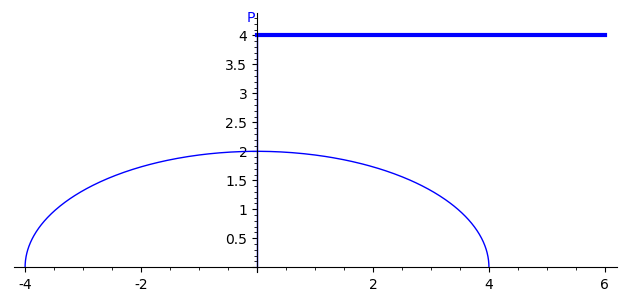
\includegraphics[scale=0.5]{sections/tmp_DSBM_N.png}
\caption{a)}
\end{center}
 \end{figure}
  

 
 \item
 Determine os valores de $m$ para os quais a reta
$$y=\frac{5}{2}x+m$$
\'e tangente a hipérbole
$$\frac{x^2}{9}-\frac{y^2}{36}=1
$$
[\textit{Dica: Use derivadas. }] 
% 
\item
 Seja $P$ o pé da perpendicular baixada do foco $F$ da hipérbole
$$\frac{x^2}{a^2}-\frac{y^2}{b^2}=1$$
a uma das assíntotas. Demonstre que $\overline{PF} = b$ e $\overline{PO} =a$, onde $O$ é a origem do sistema de coordenadas.
 

\item
 Prove que toda parábola cujo eixo \'e paralelo ao eixo $y$ tem uma equação da forma
$$y=ax^2+bx+c.$$
Qual é a forma geral das equações das parábolas cujo eixo é paralelo ao eixo $x$?
 

\item
 Deduzir uma equação da parábola que contém o ponto $(1, 4)$, sabendo-se que seu eixo é paralelo ao eixo $y$ e que seu v\'ertice é o ponto $(2,3)$.
 
% 
\item
 Deduza uma equação da parábola que contém os pontos $(-1,12), (1,2),(2,0)$ 
e tem eixo pararelo ao eixo $y$.
 
% 

 

\item
   \begin{enumerate}[leftmargin=*]
  \item[a)] Prove que a reta $x-2ay_0y+x_0=0$ \'e tangente à parábola $x= ay^2$ no ponto $P(x_0,y_0)$. [\textit{Dica: Use derivadas. }] 
  \item[b)] Mostre que a perpendicular \`a tangente em $P(x_0,y_0)$ \'e bissetriz do \^angulo formado por $PF$ (onde $F$ é o foco da parábola) e a paralela ao eixo da parábola que contém $P(x_0,y_0)$.
  \end{enumerate}
 

% 

 

\item
 Um part\'icula se move de modo que no instante $t$ seu vetor posi\c{c}\~ao \'e
 $$\vec{OP}(t)=(t,4t-t^2).$$
 Determine
  \begin{enumerate}[leftmargin=*]
  \item[a)] uma equa\c{c}\~ao cartesiana da trajet\'oria da particula;
  \item[b)] o instante em que a particula se encontra mais pr\'oxima da reta $y=5$.
  \end{enumerate}

 






























% \item Determine se são verdadeiras ou falsas as seguintes afirmações.
% \begin{enumerate}[leftmargin=*]
% \item  Duas retas paralelas a uma terceira são paralelas.
% \item  Duas retas perpendiculares a uma terceira são paralelas.
% \item  Duas retas paralelas a um plano são paralelas.
% \item  Duas retas perpendiculares a um plano são paralelas.
% \item  Duas retas ou se interceptam ou são paralelas.
% \end{enumerate}

% \item[\textcolor{blue}{44-45}] Obtenha equações paramétricas para a reta que passa pelos pontos
% $P$ e $Q$ e também para o segmento de reta ligando esses pontos.
% \item 
% \begin{enumerate}[leftmargin=*]
%     \item $P(3, -2),\quad Q(5, 1)$
%     \item $P(5, -2, 1),\quad Q(2, 4, 2)$
% \end{enumerate}
% \item 
% \begin{enumerate}[leftmargin=*]
%     \item $P (-1, 3, 5), \quad Q(-1, 3, 2)$
%     \item $P (-1, 3, 5),\quad Q(-1, 3, 2)$
% \end{enumerate}
% \item[\textcolor{blue}{46-50}] Obtenha equações paramétricas da reta que satisfaz as condições dadas.

% \item A reta que passa por $(-5, 2)$ e é paralela a $\vb=2\ib - 3\jb$.
% \item A reta que é tangente ao círculo $x^2 + y^2 = 25$ no ponto $(3,-4)$.
% \item A reta que é tangente à parábola $y = x^2$ no ponto $(-2, 4)$.

% \item A reta que passa por $(-2, 0, 5)$ e é paralela à reta $x = 1 + 2t$, $y = 4 - t$, $z = 6 + 2t$.
% \item A reta que passa pela origem e é paralela à reta $x = t$, $y = -1+ t$, $z = 2$.

% \item Em que ponto a reta $x = 1 + 3t$, $y = 2 - t$ intersecta
% \begin{enumerate}[leftmargin=*]
% \begin{multicols}{3}
%     \item o eixo $x$
%     \item o eixo $y$
%     \item a parábola $y=x^2$?
%     \end{multicols}
% \end{enumerate}
% \item Encontre a intersecção da reta $x = -2$, $y = 4 + 2t$, $z = -3 + t$ com os planos $xy$ e $xz$.

% \item Determine a projeção ortogonal do ponto $P(2,-1, 3)$ sobre a reta $x=3t,\, y=-7+5t,\, z=2+2t$.


% \item Considere o triângulo de vértices $A(1,0,-2)$, $B(2,-1,-6)$ e $(-4, 5, 2)$. Determine as equações paramétricas da reta suporte da mediana relativa ao lado $BC$.

% \item Considere o triângulo de vértices  $A(3,3,3)$ , $B(0, 1, 3)$ e $C(6, 15, -3)$ . Determine as equações paramétricas da reta suporte da altura relativa ao lado $BC$.

% \item[\textcolor{blue}{56-60}] Determine a posição relativa das retas $r_1$ e $r_2$.

% \item $r_1: x = 2 + t,\, y = 2 + 3t,\, z = 3 + t$ \\ $r_2: x = 2 + s, \,y = 3 + 4s,\, z = 4 + 2s$

% \item $r_1 : x = 1 + 7t, \,y = 3 + t, \,z = 5 - 3t$\\
% $r_2 : x = 4 - s, \,y = 6, \,z = 7 + 2s$    

% \item $r_1 : x = 2 -t, \,y = 3 + 2t, \,z = 1 + t$\\
% $r_2 : x = 5 - 2s, \,y = 2+4s, \,z = 1 + 2s$ 

% \item $r_1 : x = 2 +t, \,y = -3 -t, \,z = t$\\
% $r_2 : x = \frac{1}{2}(3s + 1), \,y = s-1, \,z = \frac{1}{3}s$   
% \item $r_1 : x = 2 +t, \,y = 4 - 2t, \,z = 1 + 3t$\\
% $r_2 : x = -1 + 4s, \,y = 3-s, \,z = 2 + 2s$ 

% \item Determine a distância do ponto $A(-2,1,2)$ à reta determinada pelos pontos $P(1,2,1)$ e $Q(0,-1,3)$.
% \item Determine a medida da projeção ortogonal de $\vb=\ib + 2\jb + \kb$ sobre a reta $x=1-2t$,$y=t$, $z=-1-2t$.
% \section{Planos}
% \item Determine se são verdadeiras ou falsas as seguintes afirmações.
% \begin{enumerate}[leftmargin=*]
%     \item  Dois planos paralelos a um terceiro são paralelos.
%     \item  Dois planos perpendiculares a um terceiro são paralelos.
%     \item  Dois planos paralelos a uma reta são paralelos.
%     \item  Dois planos perpendiculares a uma reta são paralelos.
%     \item  Dois planos ou se interceptam ou são paralelos.
%     \item  Um plano e uma reta ou se interceptam ou são paralelos.
% \end{enumerate}


% \item Determine uma equação do plano nos casos citados.

% \begin{enumerate}[leftmargin=*]
% \item passa pelo ponto $P(2, 6, 1)$ e tem $\mathbf{n}= \lan 1, 4, 2\ran$ como um vetor normal. 

% \item passa pelo ponto $P(-1, -1, 2)$ e tem $\mathbf{n}= = \lan -1, 7, 6\ran$ como um vetor normal. 

% \item que passa pelos pontos $A(-2, 1, 1)$, $B(0, 2, 3)$ e $C(1, 0, -1)$.

% \end{enumerate}
% \item Determine uma equação do plano nos seguintes casos:
% \begin{enumerate}[leftmargin=*]
%     \item paralelo ao plano $2x-3y-z+5=0$ e que passa pelo ponto $P(4,-1,2)$.
%     \item perpendicular à reta $x=1-3t$, $y=5+2t$, $z=-t$ e que passa pelo ponto $P(4,-1,2)$.
%     \item determinado pelas retas  $x=1+2t$, $y=4t$, $z=-1+6t$ e  $x=s$, $y=1+2s$, $z=-2+3s$
%     \item perpendicular ao eixo $y$ e que passa pelo ponto $P(-1,0,2)$.
%     \item determinado pelo ponto $P(3,-1,2)$ e pela reta $x=t$,$y=2-t$, $z=3+2t$.
% \end{enumerate}


% \item Determine uma equação do plano determinado pelo ponto $P(3,-2,-1)$ e pela reta de intersecção dos planos
%             $x+2y+z-1=0$ e   $2x+y-z+7=0$.
% \item  Determine uma equação do plano determinado pelo ponto $P(1,2,1)$ e pela reta de intersecção dos planos $x-2y+z-3=0$ e $x=0$.

% \item Determine uma equação do plano que contém o ponto $P(2, 0, 3)$ e a reta $x = -1 + t$, $y = t$, $z = -4 + 2t$.

% \item[\textcolor{blue}{69-70}] Obtenha equações paramétricas da reta de interseção dos planos dados.

% \item $\pi_1: -2x + 3y + 7z + 2 = 0$\\
% $\pi_2: x + 2y - 3z + 5 = 0$
% \item $\pi_1: 3x - 5y + 2z = 0$\\
% $\pi_2: z=0$
% \item Determine a distância entre o ponto $P(1, -2, 3)$ e o plano $2x - 2y + z = 4$.
% \item Determine a distância entre os planos paralelos $-2x + y + z = 0$ e $6x - 3y - 3z - 5 = 0$.

% \section{Problemas Suplementares II}
% \item Mostre que a distância entre os planos paralelos 
% \begin{align*}
%     \pi_1: ax+by+cz + d_1=0\\
%     \pi_2: ax+by+cz + d_2=0
% \end{align*}
% é 
% \begin{align*}
%     D=\dfrac{|d_1-d_2|}{\sqrt{a^2+b^2+ c^2}}
% \end{align*}
% \item Se $a$, $b$ e $c$ não são todos nulos, mostre que a equação $ax + by + cz+ d = 0$ representa um plano e $\lan a, b, c\ran$ é o vetor normal ao plano.

% \item Determine uma equação do plano cujos pontos são equidistantes de $P_1(2, -1, 1)$ e $P_2(3, 1, 5)$.

% \item Determine a equação paramétrica da $r$ que passa pelo ponto $P(1,2,0)$ e é paralela à reta de intersecção dos planos $2x-y-z+1=0$ e $x+3y+2z-4=0$
% \item Suponha que $\vb_1$ e $\vb_2$ sejam vetores com $\|\vb_1\| = 2$, $\| \vb_2\| = 3$ e $\vb_1 \cdot \vb_2 = 5$. Seja $\vb_3 = \mathrm{proj}_{\vb_1} \vb_2$ , $\vb_4 = \mathrm{proj}_{\vb_2} \vb_3$, $\vb_5 = \mathrm{proj}_{\vb_3} \vb_4$  e assim por diante. Calcule $\sum_{n=1}^{\infty}\|\vb_n \|$.
% \item Determine uma equação da esfera com centro $(2, 1, -3)$ que é tangente ao plano $x - 3y + 2z = 4$.

% \item Determine a distância entre as retas reversas 
% \begin{align*}
%     r_1: & x = 1 + 7t, \, y = 3 + t, \, z = 5 - 3t\\
%     r_2: & x = 4 - s,\, y = 6,\, z = 7 + 2s
% \end{align*}
% $$.$$
\end{enumerate}
\begin{thebibliography}{99}


\bibitem{santos} DOS SANTOS, Fabiano José; FERREIRA, Silvimar Fábio.  \textbf{Geometria Analítica},  Bookman Editora, 2009.
\bibitem{anton} ANTON, Howard; BIVENS, Irl; DAVIS, Stephen. \textbf{Cálculo-Volume II-10.} Bookman Editora, 2014.
\bibitem{reis} DOS REIS, Genesio Lima; DA SILVA, Valdir Vilmar. \textbf{Geometria Analítica}. Livros Tecnicos e Cientificos, 1984.
\bibitem {james} STEWART, James. Cálculo, volume II-10. Tradução da 7ª edição norte-americana. Cengage Learning, 2013.
\end{thebibliography}

\end{document}
